\documentclass{article}

\usepackage{fullpage}
\usepackage{pdfpages}
\usepackage{hyperref}
\usepackage{titlesec}


\hypersetup{
    colorlinks,
    citecolor=black,
    filecolor=black,
    linkcolor=blue,
    urlcolor=black,
    	linktoc=all
}

\pagestyle{empty}

\newcommand{\Department}{Computer Science and Engineering}
\newcommand{\Instructor}{Faculty Name}
\newcommand{\Semester}{Fall 2013}
\newcommand{\NumStudents}{999}
\newcommand{\CourseTitle}{Course Title}
\newcommand{\CourseNumber}{CMPS XXX}

\newcommand{\GradedWork}[2]{%
\phantomsection
\addtocounter{subsection}{1}
\addcontentsline{toc}{subsection}{#1}
\includepdf[pages={-},addtotoc={1,subsubsection,2,#1 - Best,assign:#2-best}]{graded/#2-best.pdf}
\includepdf[pages={-},addtotoc={1,subsubsection,2,#1 - Average,assign:#2-average}]{graded/#2-average.pdf}
\includepdf[pages={-},addtotoc={1,subsubsection,2,#1 - Worst,assign:#2-worst}]{graded/#2-worst.pdf}
}%

\begin{document}

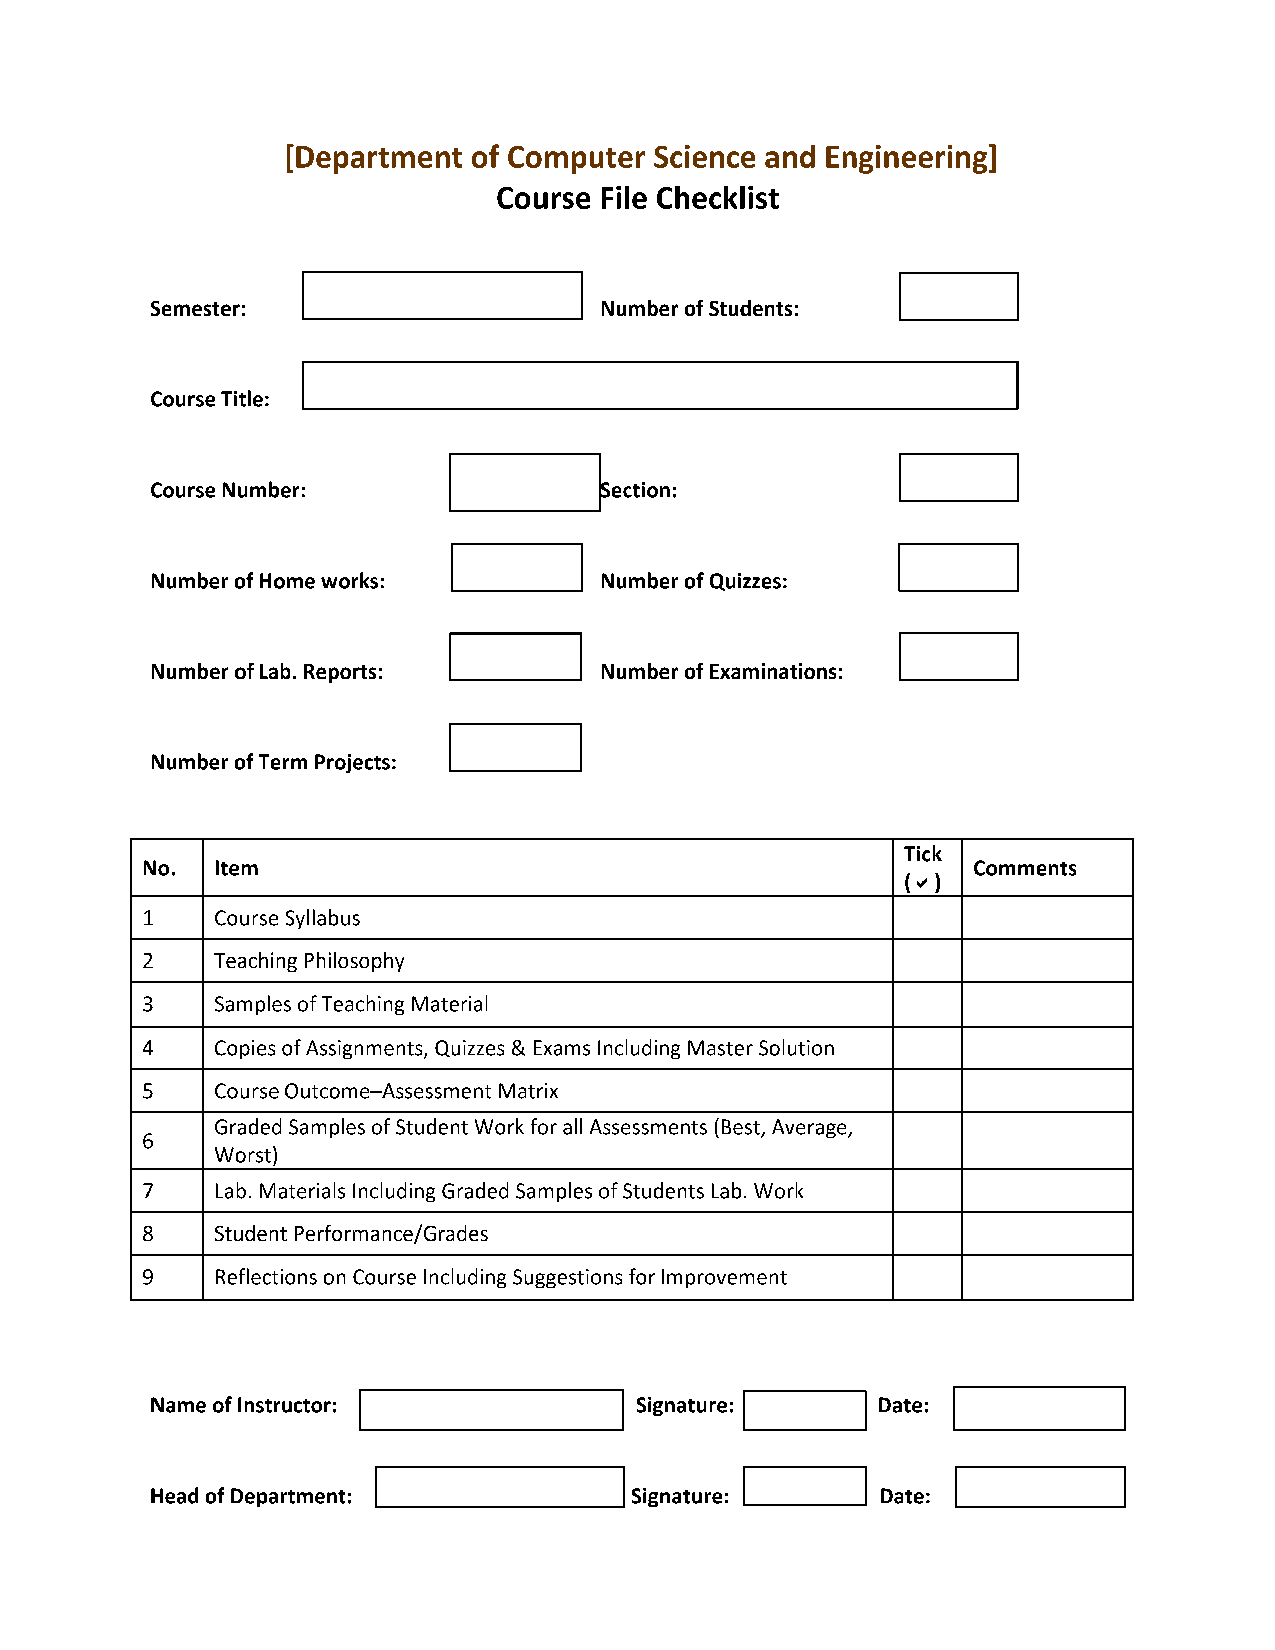
\includepdf[pages={-}]{other/checklist.pdf}

\newpage
\tableofcontents

\vspace{0.5in}


\titleformat{\section}
	{\LARGE\bfseries\centering}{}{1em}{\vfill}[\vfill]

\newpage

\section{Syllabus}
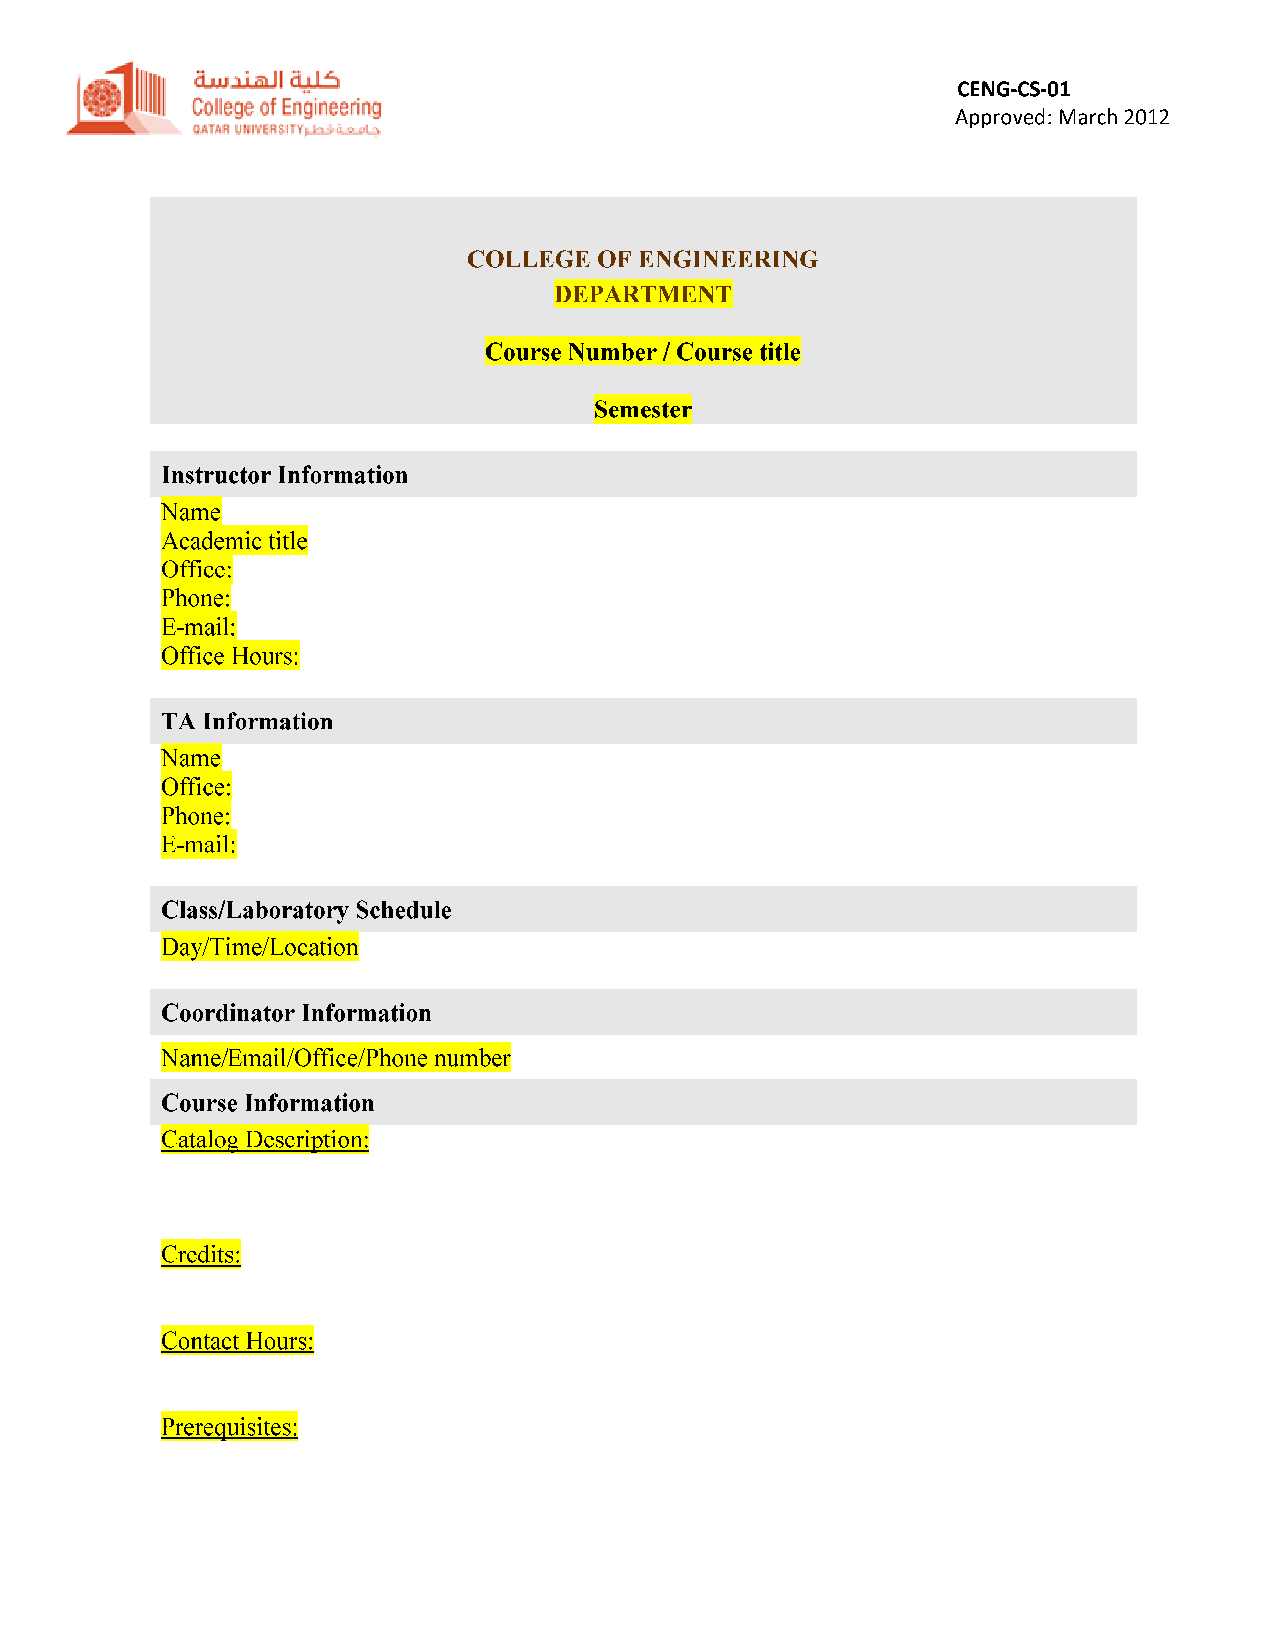
\includepdf[pages={-},addtotoc={1,subsection,2,Unified College Syllabus,syl:col}]{syllabus/syllabus.pdf}


\section{Teaching Philosophy}

\includepdf[pages=-]{other/teachingphil.pdf}

\newpage
\section{Samples of Teaching Material}

\includepdf[pages={-},addtotoc={1,subsection,2,Lecture 1: Topic,lec:01}]{lectures/lec01.pdf}

%\includepdf[pages={-},addtotoc={1,subsection,2,Lecture 2: Topic,lec:02}]{lectures/lec02.pdf}

%Add more lines like the above to add more material.

\newpage
\section{Copies of Assignments}
\newpage


\includepdf[pages={-},addtotoc={1,subsection,2,Homework 1,assign:hw1}]{coursework/hw1.pdf}


\includepdf[pages={-},addtotoc={1,subsection,2,Homework 2,assign:hw2}]{coursework/hw2.pdf}


\includepdf[pages={-},addtotoc={1,subsection,2,Midterm Exam,assign:midterm}]{coursework/midterm.pdf}


\includepdf[pages={-},addtotoc={1,subsection,2,Final Exam,assign:final}]{coursework/final.pdf}


\section{Course Outcome-Assessment Matrix}
\newpage
\subsection*{Matrix}
\begin{center}
\begin{tabular}{|l|l|l|}
\hline
			& \textbf{CO-XXX-1} & \textbf{CO-XXX-2} \\
\hline			
\textbf{Homework 1}	&	& \\
\hline
\textbf{Homework 2}	& Code & \\
\hline
\textbf{Midterm Exam	}&  & \\
\hline
\textbf{Final Exam}	& Q3, Q4(b), Q8 & \\
\hline
\end{tabular}
\end{center}


\newpage
\section{Graded Work Samples}
%\GradedWork is a helper function to automatically full in the best, average, and worst of an assignment.
%To use it for hw1, you need graded/hw1-average.pdf, graded/hw1-best.pdf, graded/hw1-worst.pdf

\GradedWork{Homework 1}{hw1}
%\GradedWork{Homework 1}{hw2}
%\GradedWork{Midterm}{midterm}
%\GradedWork{Final}{final}

\section{Lab Materials}

\begin{center}
\textbf{If your course has a lab, include its material here.}
\end{center}

\newpage
\section{Student Performance/Grades}

\includepdf[pages={-}]{other/grades.pdf}

\newpage
\section{Reflections on Course}

\includepdf[pages={-}]{other/reflect.pdf}

\end{document}